\chapter{Theory}
\label{chap:theory}

\chapterquote{The career of a young theoretical physicist consists of treating the harmonic oscillator in ever-increasing levels of abstraction.}{Sidney Coleman}

\section{Introduction}
Modern particle theory is built upon the twin pillars of Yang-Mills theories and spontaneous symmetry breaking. 
Our best current model, the Standard Model (SM), is built from two such theories: electroweak theory and quantum chromodynamics, of which the former has its gauge symmetry spontaneously broken. 
In this chapter we will explore these two ideas before moving on to how they are used to construct the Standard Model with particular emphasis on the mechanism of symmetry breaking in the SM and its phenomenological consequences. 







\section{Yang-Mills Theories}
(Some introductory words)

\subsection{From Geometry to Gauge Fields}
The gauge covariant derivative $D_{\mu}$ and the field strength tensor $F_{\mu\nu}$ are two vital mathematical objects when one wants to construct the Lagrangian of a Yang-Mills theory.
Far from simply being an ansatz, they have a deep and elegant origin in the fundamental geometry of field theory. 
Their origin is outlined in this section: we start by describing the concept of a fibre bundle, its relationship to the internal symmetries of a field, and how the `warping' of a fibre bundle is related to the covariant derivative and the field strength tensor.


A fibre bundle $\mathcal{B}$ is a space which can be considered to consist of two parts: the base space $\mathcal{M}$ and the fibre $\mathcal{V}$. For each point $p$ in the base space there is an associated copy of the fibre space and these fibres do not intersect. 
In the context of a field one can consider these to be the external and internal spaces respectively. A special case is an ordinary product space where $\mathcal{B}$ is simply the Cartesian product of $\mathcal{M}$ and $\mathcal{V}$, generally one has more warped examples with curvature and less trivial topology. A visual example is given in figure X.
These warped examples are of interest in gauge theory, specifically when there is curvature in the fibre space with no torsion.


Particularly, we are interested in the cases when $\mathcal{V}$ is symmetric under some Lie group $\mathcal{G}$ which in our field of interest will be $\SUN$. 
These symmetries allow for the warping of the fibre bundle and correspond to the internal symmetries of a field. 
Furthermore, one can model these examples by taking the fibre to be $\mathcal{G}$ with the identity element not at a fixed location. 
The relevance of this will be apparent when we consider a fibre bundle section. A bundle section can be considered to `lift' the base space into the bundle: for each base space point we get a point within the associated fibre. In the gauge theory context choosing a section of the fibre bundle means choosing a particular $g(x)\in\mathcal{G}$, this is picking a gauge. 



To understand the warping of the fibre bundle we need the notion of a connection just like with the warped spaces of General Relativity.
This will allow for the introduction of warping to the internal space, and construction of invariants such as curvature and torsion tensors.
We can do this by constructing a differential operator $D_{\mu}$, and in our case of a fibre bundle with $\mathcal{V}=\mathcal{G}=\SUN$ and the internal space is simply stretched with no torsion we have,
\begin{equation}
\label{eq:theory:g_connection}
D_{\mu} = \partial_{\mu} - igA_{\mu}^{a} T^{a}.
\end{equation}
Where $A_{\mu}^{a}$ are generally complex-valued functions which depend on $x_{\mu}$ and operate by multiplying the input, and $T^{a}$ are the generators of the Lie group $\SUN$ which provide a basis in the fibre space with $a = 0,\ldots,N^{2}-1$.
We recognise this as having the familiar form of the gauge covariant derivative and the $A_{\mu}^{a}$ as the gauge potential. 


Now we have the connection we can begin to construct invariants of the geometry of the internal space. In particular we can construct the curvature tensor as follows
\begin{equation}
    \label{eq:theory:g_curvature}
    \frac{i}{g}[D_{\mu},D_{\nu}] = F_{\mu\nu} = \partial_{\mu} A^{b}_{\nu} T^{b} - \partial_{\nu} A^{a}_{\mu} T^{a} - ig[A^{a}_{\mu}, A^{b}_{\nu}].
\end{equation}
We recognise this form as the field strength tensor.

One can now see what occurs when a global symmetry is promoted to a gauge symmetry: we have induced some non-trivial warping of the field's internal space which gives rise to the $A^{a}_{\mu}$ gauge fields and their kinematics through the curvature $F_{\mu\nu}$.




\subsection{Constructing a Lagrangian}
With these ingredients we can construct a generic Yang-Mills Lagrangian with a straightforward procedure: we begin with a global symmetry of the fields which we promote to a gauge symmetry, we construct the gauge covariant derivative, replace $\partial_{\mu} \rightarrow D_{\mu}$ in the free theory, and add an interaction term based on the field strength tensor. 
Let us consider, as a concrete example, the collection of massive free Dirac fermions which we will turn into an interacting gauge theory with $\mathcal{G} = \SUN$.
We first construct the gauge covariant derivative, 
\begin{equation}
    \label{eq:theory:generic_SUN_Dmu}
    D_{\mu} = \partial_{\mu} - igA_{\mu}^{a} T^{a},
\end{equation}
and replace $\partial_{\mu} \rightarrow D_{\mu}$ in the free Lagrangian
\begin{equation}
    \label{eq:theory:int_dirac_no_gauge_dynamics}
    \mathcal{L} = \sum_{\alpha} \bar{\Psi}^{\alpha}[i\gamma^{\mu}(D_{\mu}\Psi)^{\alpha} - m\Psi^{\alpha}].
\end{equation}
We must also introduce a kinematic term for the gauge fields, but the contraction of the general non-Abelian field strength tensor with itself is not gauge invariant, only its trace over the generator indices is. 
We us this as the gauge-invariant kinetic for our final Yang-Mills Lagranian,
\begin{equation}
    \label{eq:theory:int_dirac_gauge_dynamics}
    \mathcal{L}_{YM} = \sum_{\alpha} \bar{\Psi}^{\alpha}[i\gamma^{\mu}(D_{\mu}\Psi)^{\alpha} - m\Psi^{\alpha}] - \frac{1}{2}\mathrm{Tr}F_{\mu\nu}F^{\mu\nu}.
\end{equation}
%
%

\subsection{Phenomenology}
To analyse what sort of particle interactions occur in this theory let us `unpack' equation \ref{eq:theory:int_dirac_gauge_dynamics} and isolate the fields and interaction terms. 
Firstly, in the spectrum of this theory we have $N^{2}-1$ gauge fields (one for each of the generators of $\SUN$) which are all massless. 
These fields couple to the massive fermionic fields via a trilinear interaction term proportional to $g$ introduced by the gauge covariant derivative.
\begin{equation}
    \mathcal{L}_{{A}\Psi} = gA_{\mu}^{a}\bar{\Psi}^{\alpha}\gamma^{\mu}(T^{a})_{\alpha\beta}\Psi^{\beta}
\end{equation}
Now consider the gauge field kinetic term: one can reformulate this as $-\frac{1}{4}F^{a}_{\mu\nu}F^{a\mu\nu}$ using $\mathrm{Tr}T^{a}T^{b} = \frac{1}{2}\delta^{a}_{b}$ and $F_{\mu\nu} = F^{a}_{\mu\nu}T^{a}$. 
Once the product has been evaluated one finds the following forms of interaction terms
\begin{equation}
    \mathcal{L}_{3A} \propto gf^{abc}(\partial_{\mu}\eta_{\nu\lambda}A^{\lambda{a}})A^{b\mu}A^{c\nu} 
\end{equation}
%
\begin{equation}
    \mathcal{L}_{4A} \propto g^{2}f^{abc}f^{ade}A_{\mu}^{b}A_{\nu}^{c}A_{\lambda}^{d}A_{\sigma}^{e}
\end{equation}
%
which correspond to interactions between three and four gauge bosons respectively. 
We now have the three types of interaction vertices which allow for the construction of Feynman diagrams for a generic Yang-Mills theory (Figure \ref{fig:theory:YM-vertices}). 
Their strengths are all set in terms of a single parameter: the gauge coupling $g$.
One should note that the three and four-gauge boson interactions come from the commutator in the gauge field kinematic term and are not present in the Abelian case. 




\begin{figure}[h!]
    \begin{center}
        \begin{tikzpicture}[baseline=(current bounding box.center)]
        \begin{feynman}
            \vertex (a) {\(A^{a}_{\mu}\)};
            \vertex [right=of a] (b);
            \vertex [above right=of b] (f1) {\(\Psi^{\beta}\)};
            \vertex [below right=of b] (f2) {\(\bar{\Psi}^{\alpha}\)};
            \diagram* {
                (a) -- [boson] (b) -- [fermion] (f1),
                (f2) -- [fermion] (b),
            };
        \end{feynman}
        \end{tikzpicture}
        %
        \qquad
        \begin{tikzpicture}[baseline=(current bounding box.center)]
        \begin{feynman}
            \vertex (a) {\(A^{a}_{\mu}\)};
            \vertex [right=of a] (b);
            \vertex [above right=of b] (f1) {\(A^{b}_{\nu}\)};
            \vertex [below right=of b] (f2) {\(A^{c}_{\lambda}\)};
            \diagram* {
                (a) -- [boson] (b) -- [boson] (f1),
                (b) -- [boson] (f2),
            };
        \end{feynman}
        \end{tikzpicture}
        %
        \qquad
        \begin{tikzpicture}[baseline=(current bounding box.center)]
        \begin{feynman}
            \vertex (b);
            \vertex [above left=of b] (a) {\(A^{a}_{\mu}\)};
            \vertex [below left=of b] (c) {\(A^{b}_{\nu}\)};
            \vertex [above right=of b] (f1) {\(A^{c}_{\lambda}\)};
            \vertex [below right=of b] (f2) {\(A^{d}_{\sigma}\)};
            \diagram* {
                (a) -- [boson] (b), 
                (b) -- [boson] (f1),
                (b) -- [boson] (c),
                (b) -- [boson] (f2),
            };
        \end{feynman}
        \end{tikzpicture}
    \end{center}
    \caption{The three types of vertex in Yang-Mills theories.}
    \label{fig:theory:YM-vertices}
\end{figure}



\section{Spontaneous Symmetry Breaking}
Spontaneous symmetry breaking (SSB) occurs when the lowest energy solutions to a theory do not respect the symmetries of the Lagrangian which describes it. 
A straightforward example is that of a three-dimensional ferromagnetic material which is cooling down from above its Curie temperature.
Above this threshold there is no magnetisation and solutions obey the $\mathrm{SO}(3)$ symmetry of the Lagranian, 
below this threshold the ferromagnet becomes magnetised and must `choose' one of a degenerate family of lowest-energy solutions. This picks out a direction of magnetisation. The $\mathrm{SO}(3)$ symmetry of the ferromagnet has now been broken to $\mathrm{SO}(2)$.

\begin{figure}[h!]
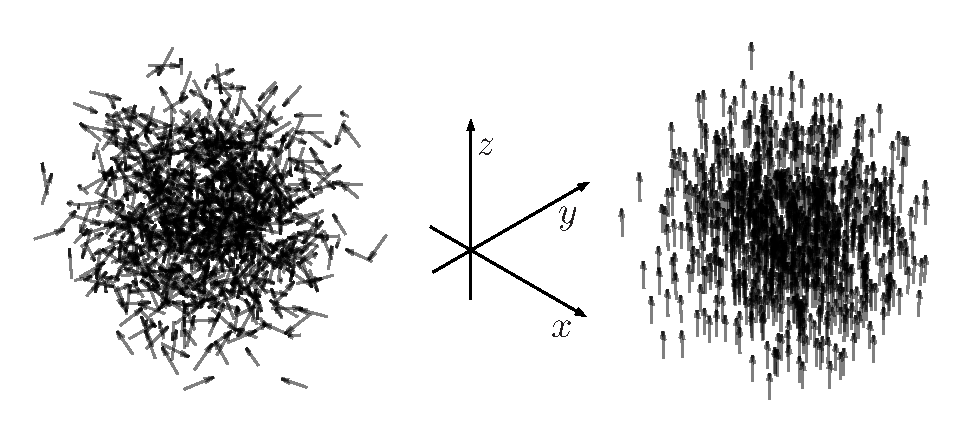
\includegraphics[width=0.9\textwidth]{figures/theory/ferromagnet_ssb.pdf}
\caption{A ferromagnet above (left) and below (right) the Curie temperature. The example below the Curie temperature has magnetised along the z-direction breaking the $\mathrm{SO}(3)$ symmetry to just $\mathrm{SO}(2)$ about the z-axis}
\label{fig:theory:ferromagnet_ssb}
\end{figure}

In the context of a field theory symmetry can be spontaneously broken in the following way: a field experiences a potential whose minima are a family of degenerate states transforming under the symmetry group. 
Consider the case of a complex scalar field $\phi$ with the following Lagrangian,
\begin{equation}
    \label{eq:theory:global_SSB_L}
    \mathcal{L} = \partial_{\mu}\phi^{*}\partial^{\mu}\phi - \frac{1}{2}\lambda^{2}(|\phi|^{2} - \eta^{2})^{2}.
\end{equation}

\begin{figure}[h!]
    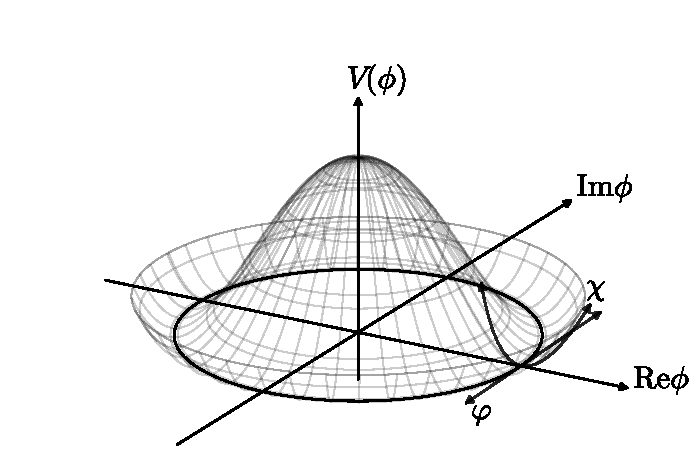
\includegraphics[width=0.65\textwidth]{figures/theory/ssb_potential.pdf}
    \caption{placeholder.}
    \label{fig:theory:global_ssb_potential}
\end{figure}
This has a global $\mathrm{U}(1)$ symmetry, $\phi\rightarrow|\phi|e^{i\theta}$, and a potential with a family of degenerate minima at $|\phi| = \eta$. The vacuum expectation values (VEVs) of $\phi$, $\langle\phi\rangle$ form a circle of radius $\eta$ and their location on this circle is parameterised by $\langle\theta\rangle$ which can take any value $\theta_{0}$. The field will settle into one of these vacuum states and the global symmetry is spontaneously broken.

To see the effects of this SSB let us consider a small perturbation around the vacuum with $\theta_{0}=0$. We describe $\phi$ in terms of two real scalar fields: one along the imaginary direction of $\phi$ and one along the real,
\begin{equation}
    \phi(x) = \eta + (\chi(x) + i\varphi(x)).
\end{equation}
If one substitutes this into equation \ref{eq:theory:global_SSB_L} we find that
\begin{equation}
    \mathcal{L} = \partial_{\mu}\chi\partial^{\mu}\chi + \partial_{\mu}\varphi\partial^{\mu}\varphi - \frac{1}{2}\lambda^{2}(2\eta\chi + \chi^{2} + \varphi^{2})^{2} 
\end{equation}
and if one evaluates the non-kinematic part we find that the field $\chi$ is granted a mass term of the form $\frac{1}{2}m^{2}\chi^{2}$,
\begin{equation}
    \frac{1}{2}m_{\chi}^{2}\chi^{2} = 2\lambda^{2}\eta^{2}\chi^{2}
\end{equation}
and there is no equivalent term for $\varphi$. In the spectrum of this theory we now have a massive and a massless scalar boson upon quantisation. This massless boson is known as a Goldstone boson and is a general result of breaking a global symmetry: for each broken symmetry generator there is a massless Goldstone boson. 

In the non-Abelian case, the family of vacua transform into each other under the group of higher dimensionality. The scalar field that transforms under this larger group non-trivially must have more components and as a result so will the family of vacua: one for each group generator. Once the symmetry is broken there is a massless field for each of these generators. 

\subsection{Gauge Symmetry Breaking}
In the case where we have a gauge symmetry that is spontaneously broken the behaviour is rather different: there are no Goldstone bosons and the gauge bosons are granted mass. 
Let us take the example of equation \ref{eq:theory:global_SSB_L} and promote the global $\mathrm{U}(1)$ symmetry to a gauge symmetry: we construct the gauge-covariant derivative
%
\begin{equation}
    \label{eq:theory:gauge_cov_deriv_u1}
    D_{\mu} = \partial_{\mu} + igA_{\mu},
\end{equation}
%
use it to replace the partial derivative, and introduce a gauge field kinetic term to get the gauge-invariant Lagrangian
\begin{equation}
    \label{eq:theory:gauge_u1_lagrangian}
    \mathcal{L} = (D_{\mu}\phi)^{*}(D^{\mu}\phi) - \frac{1}{2}\lambda^{2}(|\phi|^{2} - \eta^{2})^{2} - \frac{1}{4}F_{\mu\nu}F^{\mu\nu}.
\end{equation}
%
We can consider the field $\phi$ in terms of its modulus and a phase, and then expand around $\eta$,
\begin{equation}
    \label{eq:theory:phi_decomposition}
    \phi(x) = |\phi(x)|e^{i\alpha(x)} = (\eta + \frac{1}{\sqrt{2}}\varphi(x))e^{i\alpha(x)}
\end{equation}
where $\varphi$ is a real scalar field corresponding to the direction orthogonal to the family of vacua and $\alpha$ corresponds to the direction along it. 
We recognise that the phase can always be removed by some gauge transformation $\exp(-i\alpha(x))$, so we can freely set it to zero. 
We have removed one degree of freedom and we only have only one real scalar left: the gauge freedom has eliminated the Goldstone boson from the spectrum of the theory.


When we substitute equation \ref{eq:theory:phi_decomposition} into the Lagrangian \ref{eq:theory:gauge_u1_lagrangian} and then collect the terms which contain $A_{\mu}$ we get the following Lagrangian for the gauge field (neglecting interaction terms)
\begin{equation}
    \label{eq:theory:abelian_gaugefield_L}
    \mathcal{L}_{A} = -\frac{1}{4}F_{\mu\nu}F^{\mu\nu} + g^{2}\eta^{2}A_{\mu}A^{\mu} %+ g^{2}\frac{2}{\sqrt{2}}\eta\varphi A_{\mu}A^{\mu} + g^{2}\frac{1}{2}\varphi^{2}A_{\mu}A^{\mu} 
\end{equation}
This contains a mass terms of the form $\frac{1}{2}m_{A}^{2}A_{\mu}A^{\mu}$, we conclude that the field $\alpha(x)$ has indeed been eliminated and that this degree of freedom has been absorbed into the longitudinal component of the gauge field $A_{\mu}$ which has been granted mass $m_{A}^{2}=2g^{2}\eta^{2}$. 


Collecting the scalar field $\varphi$ terms in the same way we have 
\begin{equation}
    \label{eq:theory:abelian_scalar_SSB_L}
    \mathcal{L}_{\varphi} = \frac{1}{2}(\partial_{\mu}\varphi)(\partial^{\mu}\varphi) - \lambda^{2}\eta^{2}\varphi^{2}% - \frac{1}{sqrt{2}} 
\end{equation}
and we conclude that the theory contains a massive scalar field with $m_{\varphi}^{2} = 2\eta^{2}\lambda^{2}$ as in the global case. Upon quantisation fields such as $\varphi$ are called Higgs bosons, and these fields have far-reaching consequences for theories of fundamental physics playing a crucial role in the Standard Model by granting mass to all the fundamental field quanta such as electrons and quarks and by breaking part of the gauge symmetry group of the Standard Model. 










\section{The Standard Model of Particle Physics}
Overview
\subsection{The Electroweak Interaction}
Strategy of this subsection

\subsubsection{Gauge Bosons, the Higgs Field, and Symmetry Breaking}
Consider a Yang-Mills theory consisting of a complex scalar $\mathrm{SU}(2)$ doublet $\phi$ 
\begin{equation}
    \label{eq:theory:higgs_doublet}
    \phi = \begin{pmatrix}
        \phi^{+} \\
        \phi^{0}
    \end{pmatrix}
\end{equation}
and a symmetry group $\mathcal{G}=\mathrm{SU}(2)\times\mathrm{U}(1)$ experiencing a potential $V(|\phi|)$. We build the gauge-covariant derivative 
\begin{equation}
    \label{eq:theory:electroweak_cov_deriv}
    D_{\mu} = \partial_{\mu} \frac{ig}{2}\tau^{a}W_{\mu}^{a} + \frac{ig^{'}}{2}B_{\mu}\mathbb{1}
\end{equation}
where $W_{\mu}^{a}$ are the gauge fields corresponding to each of the generators of the $\mathrm{SU}(2)$ subgroup of $\mathcal{G}$, the $\tau^{a}$ are the $\mathrm{SU}(2)$ generators (Pauli Matrices), $B_{\mu}$ is the gauge field corresponding to the Abelian subgroup $\mathrm{U}(1)$, and $g$,$g^{'}$ are the gauge couplings corresponding to the $\mathrm{SU}(2)$ and $\mathrm{U}(1)$ respectively. 
The internal field space here has two complex dimensions and the internal geometry corresponds to unit circle in the 2D complex space ($\mathrm{SU}(2)$) warped by a position-dependent complex phase ($\mathrm{U}(1)$).
Both the third component of the $\mathrm{SU}(2)$ gauge field and $B_{\mu}$ both multiply a diagonal matrix in the internal isospin space and will later need to be unmixed. 


We construct the following Lagrangian for the complex scalar theory
\begin{equation}
    \label{eq:theory:electroweak_scalar_lagrangian}
    \mathcal{L} = (D_{\mu}\phi)^{\dag}(D_{\mu}\phi) - V(\phi) - \frac{1}{2}\mathrm{Tr}F_{\mu\nu}F^{\mu\nu} - \frac{1}{4}G_{\mu\nu}G^{\mu\nu}
\end{equation}
where $G_{\mu\nu} = \partial_{\mu}B_{\nu} - \partial_{\nu}B_{\mu}$ is the Abelian field strength tensor, $\phi$ experiences a potential $V(\phi)$ of the form
\begin{equation}
    \label{eq:theory:electroweak_higgs_potential}
    V(\phi) = -\mu^{2}\phi^{\dag}\phi + \lambda(\phi^{\dag}\phi)^{2}. 
\end{equation}
When $\mu^{2} > 0$ $\phi$ adopt a ground state from the family of minima and gain a non-zero vacuum expectation value (VEV) and the $\mathrm{SU}(2)$ subgroup is broken. As in the Abelian case described previously, 



\subsubsection{Leptons}

\subsubsection{Hadrons}

\subsection{Strong Interaction}

